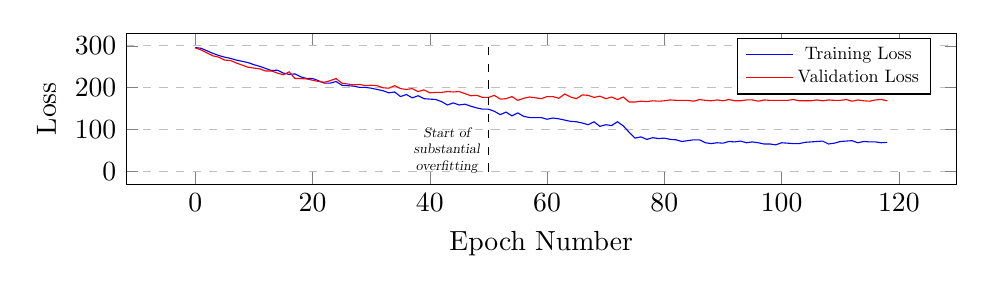
\begin{tikzpicture}
    \begin{axis}[
                height=3.5cm,
                width=\linewidth,
                xlabel={Epoch Number},
                ylabel={Loss},
                legend pos=north east,
                ymajorgrids=true,
                grid style=dashed,
                legend style={nodes={scale=0.65, transform shape}},
            ]
        %
        % TRAINING LOSS
        %
        \addplot[color=blue] coordinates {
            (0, 296) (1, 294) (2, 288) (3, 282) (4, 277) (5, 273) (6, 270) (7,
            266) (8, 263) (9, 260) (10, 255) (11, 251) (12, 246) (13, 241) (14,
            242) (15, 235) (16, 232) (17, 233) (18, 226) (19, 222) (20, 222)
            (21, 217) (22, 211) (23, 211) (24, 215) (25, 206) (26, 205) (27,
            204) (28, 201) (29, 201) (30, 199) (31, 196) (32, 193) (33, 188)
            (34, 190) (35, 179) (36, 184) (37, 176) (38, 181) (39, 174) (40,
            173) (41, 172) (42, 167) (43, 159) (44, 164) (45, 159) (46, 161)
            (47, 156) (48, 152) (49, 149) (50, 149) (51, 144) (52, 136) (53,
            142) (54, 133) (55, 140) (56, 132) (57, 129) (58, 129) (59, 129)
            (60, 125) (61, 128) (62, 126) (63, 123) (64, 120) (65, 119) (66,
            116) (67, 112) (68, 119) (69, 108) (70, 112) (71, 110) (72, 119)
            (73, 109) (74, 94) (75, 80) (76, 83) (77, 77) (78, 81) (79, 79) (80,
            80) (81, 77) (82, 76) (83, 72) (84, 74) (85, 76) (86, 76) (87, 69)
            (88, 67) (89, 69) (90, 68) (91, 72) (92, 71) (93, 73) (94, 69) (95,
            71) (96, 69) (97, 66) (98, 66) (99, 64) (100, 69) (101, 68) (102,
            67) (103, 67) (104, 70) (105, 71) (106, 72) (107, 73) (108, 66)
            (109, 68) (110, 72) (111, 73) (112, 74) (113, 69) (114, 72) (115,
            71) (116, 71) (117, 69) (118, 70)
        };
        \addlegendentry{Training Loss}
        %
        % VALIDATION LOSS
        %
        \addplot[color=red] coordinates {
            (0, 295) (1, 290) (2, 283) (3, 276) (4, 273) (5, 266) (6, 265) (7,
            259) (8, 254) (9, 249) (10, 247) (11, 245) (12, 240) (13, 240) (14,
            235) (15, 231) (16, 238) (17, 222) (18, 222) (19, 221) (20, 218)
            (21, 215) (22, 213) (23, 217) (24, 222) (25, 211) (26, 209) (27,
            207) (28, 208) (29, 205) (30, 206) (31, 205) (32, 200) (33, 199)
            (34, 205) (35, 198) (36, 196) (37, 198) (38, 191) (39, 195) (40,
            188) (41, 189) (42, 189) (43, 191) (44, 190) (45, 191) (46, 186)
            (47, 181) (48, 182) (49, 177) (50, 177) (51, 182) (52, 173) (53,
            174) (54, 179) (55, 170) (56, 175) (57, 178) (58, 176) (59, 174)
            (60, 179) (61, 179) (62, 175) (63, 185) (64, 178) (65, 174) (66,
            183) (67, 182) (68, 177) (69, 180) (70, 174) (71, 178) (72, 172)
            (73, 178) (74, 166) (75, 166) (76, 168) (77, 167) (78, 169) (79,
            168) (80, 169) (81, 171) (82, 170) (83, 170) (84, 170) (85, 168)
            (86, 172) (87, 170) (88, 169) (89, 171) (90, 169) (91, 172) (92,
            169) (93, 169) (94, 171) (95, 171) (96, 168) (97, 171) (98, 170)
            (99, 170) (100, 170) (101, 170) (102, 172) (103, 169) (104, 169)
            (105, 169) (106, 171) (107, 169) (108, 171) (109, 170) (110, 170)
            (111, 172) (112, 168) (113, 171) (114, 169) (115, 168) (116, 171)
            (117, 172) (118, 169) 
        };
        %
        % OVERFITTING LINE
        %
        \addplot[mark=none, dashed] coordinates {(50, 0) (50, 300)}
            node[midway, scale=0.5, yshift=-3em, xshift=-3em] {
                \parbox{5em}{\slshape\centering%
                    Start of substantial overfitting}
            };
        \addlegendentry{Validation Loss}
    \end{axis}
\end{tikzpicture}

